Kako bi se opisani modeli mogli bolje usporediti na problemu detekcije ljudi, potrebno ih je evaluirati na različitim skupovima podataka. U nastavku su opisani korišteni skupovi.

\section{INRIA Person}
Skup podataka INRIA person sastoji se od slika različitih veličina iz gradova i prirode. Skup za trening se sastoji od 1834 slike od kojih je 615 pozitivnih primjera (barem jedna osoba se nalazi na slici) i 1219 negativnih (nijedna osoba se ne nalazi na slici) primjera. Skup za testiranje se sastoji od 743 slike od kojih je 289 pozitivnih i 454 negativne.
Na pozitivnim primjerima ljudi su u prvom planu i zauzimaju barem 100 piksela slike po visini.

\begin{figure}[H]
\subfloat{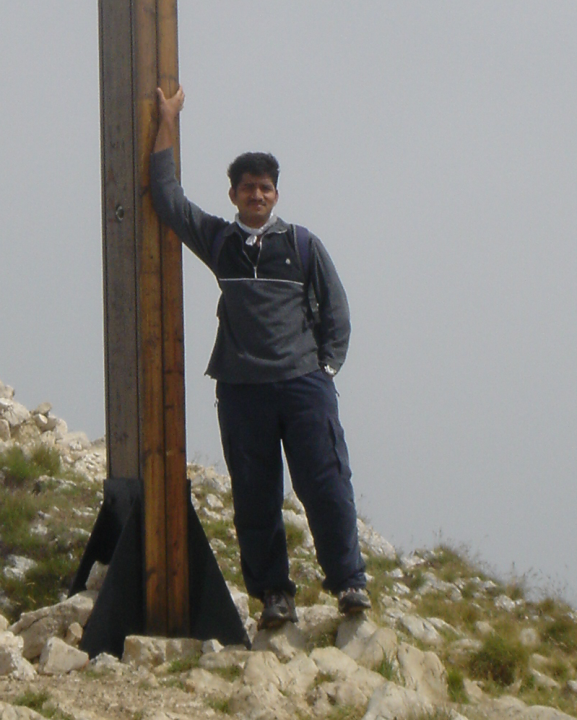
\includegraphics[height = 1.7in]{img/INRIA/crop_000012}} \
\subfloat{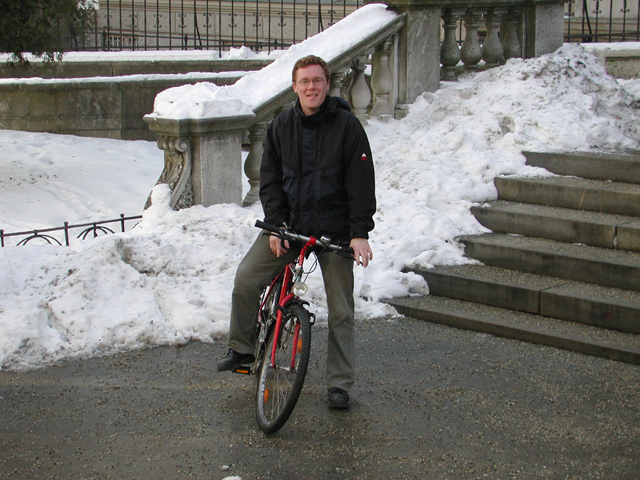
\includegraphics[height = 1.7in]{img/INRIA/person_and_bike_161}} \
\subfloat{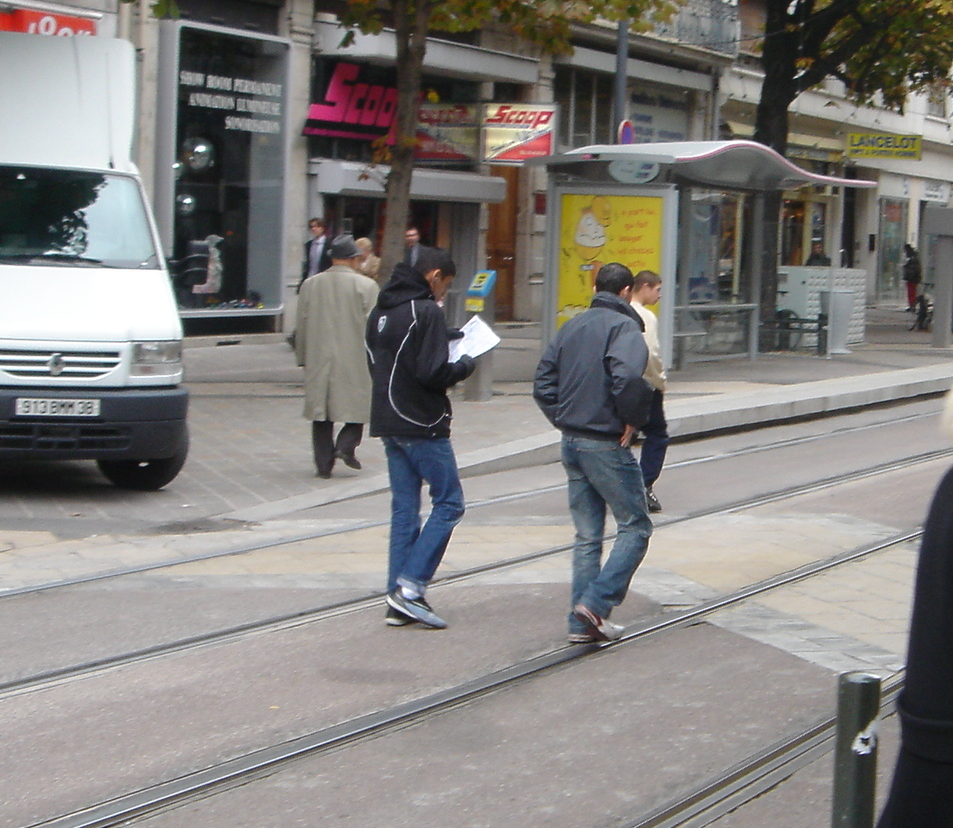
\includegraphics[height = 1.7in]{img/INRIA/crop001514}}
\caption{Primjeri slika iz INRIA Person skupa podataka.}
\end{figure}

\section{PeopleArt}
PeopleArt, \cite{westlake2016detecting}, je skup podataka koji se sastoji od fotografija i umjetničkih slika na kojima se nalaze ljudi. Slike su podijeljene u 43 kategorije. 41 kategorija je preuzeta s WikiArt.org stranice, kategorija "photos" je preuzeta iz PASCAL VOC 2012 skupa podataka, a slike iz "cartoons" kategorije su preuzete s Google-a.
Skup za testiranje se sastoji od ukupno 1616 slika (522 pozitivne i 1094 negativne).

\begin{figure}[H]
\subfloat{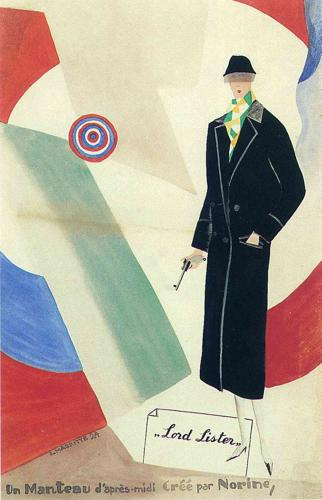
\includegraphics[height = 1.8in]{img/people-art/rene-magritte_advertisment-for-norine-2.jpg}} \
\subfloat{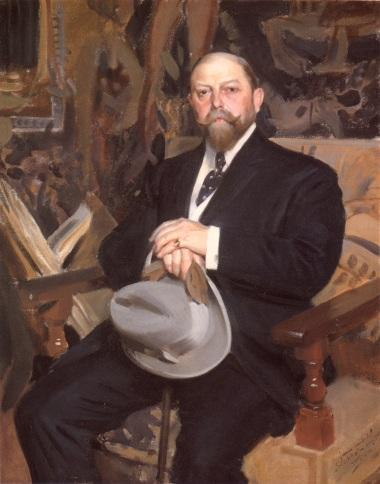
\includegraphics[height = 1.8in]{img/people-art/anders-zorn_hugo-reisinger-1907.jpg}} \
\subfloat{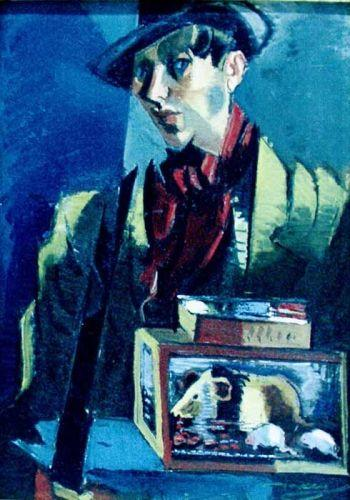
\includegraphics[height = 1.8in]{img/people-art/m-h-maxy_organ-grinder-1940.jpg}} \
\subfloat{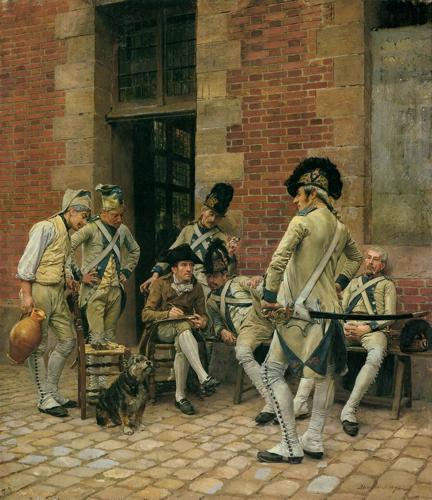
\includegraphics[height = 1.8in]{img/people-art/ernest-meissonier_the-portrait-of-a-sergeant-1874.jpg}}
\caption{Primjeri slika iz PeopleArt skupa podataka.}
\end{figure}

\section{COCO}
COCO (Common Objects in Context), \cite{DBLP:journals/corr/LinMBHPRDZ14}

\section{Nogometne utakmice}